%! Author = sebash
%! Date = 6/21/22

\documentclass{article}
\usepackage{blindtext}
\usepackage{amsmath, amssymb}
\usepackage[makeroom]{cancel}
\usepackage{pgfplots}
\usepgfplotslibrary{fillbetween}
\usepackage{tikz}
\usetikzlibrary{calc,shapes, arrows}
\usepackage{sectsty}
\usepackage{amssymb}


\newcommand{\tikzmark}[1]{\tikz[overlay,remember picture] \node (#1) {};}
\newcommand{\DrawBox}[2]{%
    \begin{tikzpicture}[overlay,remember picture]
        \draw[->,shorten >=5pt,shorten <=5pt,out=70,in=130,distance=0.5cm,#1] (MarkA.north) to (MarkC.north);
        \draw[->,shorten >=5pt,shorten <=5pt,out=50,in=140,distance=0.3cm,#2] (MarkA.north) to (MarkB.north);
    \end{tikzpicture}
}

\newcommand{\DrawBoxThree}[3]{%
    \begin{tikzpicture}[overlay,remember picture]
        \draw[->,shorten >=5pt,shorten <=5pt,out=70,in=130,distance=0.5cm,#1] (MarkA.north) to (MarkC.north);
        \draw[->,shorten >=5pt,shorten <=5pt,out=50,in=140,distance=0.3cm,#2] (MarkA.north) to (MarkB.north);
        \draw[->,shorten >=5pt,shorten <=5pt,out=90,in=120,distance=0.7cm,#3] (MarkA.north) to (MarkD.north);
    \end{tikzpicture}
}
\title{Sebastian Campos Homework}

\DeclareMathSizes{12}{30}{16}{12}

\begin{document}
    \maketitle
    \noindent
    \section*{2.7 (part two) 481 to 489 odd}
    \subsection*{481.}
        \begin{align*}|6x - 5| = |2x+ 3| \end{align*}
        \begin{align*}
            6x - 5 &= -2x -3 \hspace{2cm}or\hspace{.2cm} &6x -5 &= 2x + 3 \\
            6x \cancel{- 5} &= -2x -3 +5 &6x \cancel{-5} &= 2x + 3 + 5 \\
            6x &= -2x + 2 &6x &= 2x + 8 \\
            6x + 2x &= \cancel{-2x} + 2 &6x - 2x &= \cancel{2x} + 8 \\
            8x &= 2 &4x &= 8 \\
            \frac{8x}{8} &= \frac{2}{8} &\frac{4x}{4} &= \frac{8}{4} \\
            x &= \frac{1}{4} \hspace{3cm}or\hspace{.2cm} &x &= 2 \\
        \end{align*}
        \begin{align*}
            \boxed{x = \frac{1}{4}, x = 2}
        \end{align*}

    \subsection*{483.}
    \begin{align*}
        |2x - 5| + 2 &= 3\\
        |2x - 5| \cancel{+ 2} &= 3 - 2\\
        |2x - 5| &= 1\\
    \end{align*}
    \begin{align*}
        2x - 5 &= 1 \hspace{3cm}or\hspace{.2cm} &2x - 5 &= -1 \\
        2x \cancel{-5} &= 1 + 5 & 2x \cancel{- 5} &= -1 + 5\\
        2x &= 6 &2x &= 4 \\
        \frac{2x}{2} &= \frac{6}{2} &\frac{2x}{2} &= \frac{4}{2} \\
        x &= 3 \hspace{3cm}or\hspace{.2cm} &x &= 2 \\
    \end{align*}
    \begin{align*}
        \boxed{x = 3, x = 2}
    \end{align*}

    \subsection*{485.}
    \begin{align*}
        |3x + 1| - 3 &= 7\\
        |3x + 1| \cancel{- 3} &= 7 + 3\\
        |3x + 1| &= 10\\
    \end{align*}
    \begin{align*}
        3x + 1 &= 10 \hspace{3cm}or\hspace{.2cm} &3x + 1 &= -10 \\
        3x \cancel{+ 1} &= 10 - 1  &3x \cancel{+ 1} &= -10 - 1 \\
        3x &= 9 &3x &= -11 \\
        \frac{3x}{3} &= \frac{9}{3} &\frac{3x}{3} &= \frac{-11}{3} \\
        x &= 3 \hspace{3cm}or\hspace{.2cm} &x &= -\frac{11}{3} \\
    \end{align*}
    \begin{align*}
        \boxed{x = 3, -\frac{11}{3}}
    \end{align*}

    \subsection*{487.}
    \begin{align*}
        5|2x - 1| - 3 &= 7\\
        5|2x - 1| \cancel{- 3} &= 7 + 3\\
        5|2x - 1| &= 10\\
        \frac{5|2x - 1|}{5} &= \frac{10}{5}\\
        |2x - 1| &= 2\\
    \end{align*}
    \begin{align*}
        2x - 1 &= 2 \hspace{3cm}or\hspace{.2cm} &2x - 1 &= -2 \\
        2x \cancel{- 1} &= 2 + 1  &2x \cancel{- 1} &= -2 +1 \\
        2x &= 3 &2x &= -1 \\
        \frac{2x}{2} &= \frac{3}{2} &\frac{2x}{2} &= \frac{-1}{2} \\
        x &= \frac{3}{2}  \hspace{3cm}or\hspace{.2cm} &x &= -\frac{-1}{2} \\
    \end{align*}
    \begin{align*}
        \boxed{x = \frac{3}{2} , -\frac{1}{2}}
    \end{align*}

    \subsection*{489.}
    \begin{align*}
        |x - 7| &> -3\\
        |x - 7| &> \boxed{-3}
    \end{align*}
    \begin{align*}
        \boxed{Identity}
    \end{align*}

    \section*{3.1 1 and 3, 9 to 59 odd}
    \subsection*{1.}
    \begin{tikzpicture}
        \hspace{3cm}
        \begin{axis}[axis lines=middle,axis equal,grid=both]
            \addplot+[only marks, point meta=explicit symbolic, nodes near coords]
            coordinates{
                (-4,2) [a II]
                (-1,-2) [b III]
                (3, -5) [c IV]
                (-3,0) [d negative x axis]
                (1.66,2) [e I]
            };
        \end{axis}
    \end{tikzpicture}

    \subsection*{3.}
    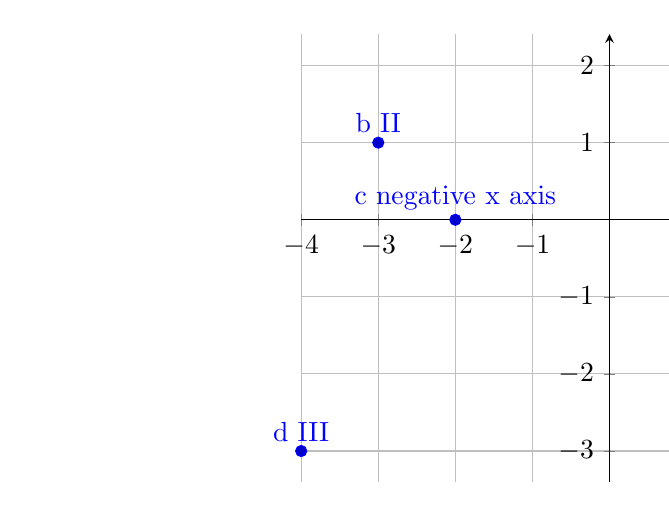
\begin{tikzpicture}
        \hspace{3cm}
        \begin{axis}[axis lines=middle,axis equal,grid=both]
            \addplot+[only marks, point meta=explicit symbolic, nodes near coords]
            coordinates{
                (3,-1) [a IV]
                (-3,1) [b II]
                (-2, 0) [c negative x axis]
                (-4,-3) [d III]
                (1.66,2) [e I]
            };
        \end{axis}
    \end{tikzpicture}
    \subsection*{9.}
    \begin{tikzpicture}
        \hspace{3cm}
        \begin{axis}[xtick distance=4, ytick distance=4, xmin=-12, xmax=12, ymin=-12, ymax=12, axis x line=middle, axis y line=middle]
            \addplot[domain=-12:12]{x+2};
        \end{axis}
    \end{tikzpicture}

    \subsection*{11.}
    \begin{tikzpicture}
        \hspace{3cm}
        \begin{axis}[xtick distance=4, ytick distance=4, xmin=-12, xmax=12, ymin=-12, ymax=12, axis x line=middle, axis y line=middle]
            \addplot[domain=-12:12]{3*x-1};
        \end{axis}
    \end{tikzpicture}

    \subsection*{13.}
    \begin{tikzpicture}
        \hspace{3cm}
        \begin{axis}[xtick distance=4, ytick distance=4, xmin=-12, xmax=12, ymin=-12, ymax=12, axis x line=middle, axis y line=middle]
            \addplot[domain=-12:12]{-x-3};
        \end{axis}
    \end{tikzpicture}

    \subsection*{15.}
    \begin{tikzpicture}
        \hspace{3cm}
        \begin{axis}[xtick distance=4, ytick distance=4, xmin=-12, xmax=12, ymin=-12, ymax=12, axis x line=middle, axis y line=middle]
            \addplot[domain=-12:12]{2*x};
        \end{axis}
    \end{tikzpicture}

    \subsection*{17.}
    \begin{tikzpicture}
        \hspace{3cm}
        \begin{axis}[xtick distance=4, ytick distance=4, xmin=-12, xmax=12, ymin=-12, ymax=12, axis x line=middle, axis y line=middle]
            \addplot[domain=-12:12]{1/2*x+2};
        \end{axis}
    \end{tikzpicture}

    \subsection*{19.}
    \begin{tikzpicture}
        \hspace{3cm}
        \begin{axis}[xtick distance=4, ytick distance=4, xmin=-12, xmax=12, ymin=-12, ymax=12, axis x line=middle, axis y line=middle]
            \addplot[domain=-12:12]{4/3*x-5};
        \end{axis}
    \end{tikzpicture}

    \subsection*{21.}
    \begin{tikzpicture}
        \hspace{3cm}
        \begin{axis}[xtick distance=4, ytick distance=4, xmin=-12, xmax=12, ymin=-12, ymax=12, axis x line=middle, axis y line=middle]
            \addplot[domain=-12:12]{-2/5*x+1};
        \end{axis}
    \end{tikzpicture}

    \subsection*{23.}
    \begin{tikzpicture}
        \hspace{3cm}
        \begin{axis}[xtick distance=4, ytick distance=4, xmin=-12, xmax=12, ymin=-12, ymax=12, axis x line=middle, axis y line=middle]
            \addplot[domain=-12:12]{-3/1*x+2};
        \end{axis}
    \end{tikzpicture}

    \subsection*{25. a}
    \begin{tikzpicture}
        \hspace{3cm}
        \begin{axis}[xtick distance=4, ytick distance=4, xmin=-12, xmax=12, ymin=-12, ymax=12, axis x line=middle, axis y line=middle]
            \addplot[domain=-12:12] coordinates {(4,12) (4,-12)};
        \end{axis}
    \end{tikzpicture}

    \subsection*{25. b}
    \begin{tikzpicture}
        \hspace{3cm}
        \begin{axis}[xtick distance=4, ytick distance=4, xmin=-12, xmax=12, ymin=-12, ymax=12, axis x line=middle, axis y line=middle]
            \addplot[domain=-12:12] {3};
        \end{axis}
    \end{tikzpicture}

    \subsection*{27. a}
    \begin{tikzpicture}
        \hspace{3cm}
        \begin{axis}[xtick distance=4, ytick distance=4, xmin=-12, xmax=12, ymin=-12, ymax=12, axis x line=middle, axis y line=middle]
            \addplot[domain=-12:12] coordinates {(-2,12) (-2,-12)};
        \end{axis}
    \end{tikzpicture}

    \subsection*{27. b}
    \begin{tikzpicture}
        \hspace{3cm}
        \begin{axis}[xtick distance=4, ytick distance=4, xmin=-12, xmax=12, ymin=-12, ymax=12, axis x line=middle, axis y line=middle]
            \addplot[domain=-12:12] {-3};
        \end{axis}
    \end{tikzpicture}

    \subsection*{29.}
    \begin{tikzpicture}
        \hspace{3cm}
        \begin{axis}[xtick distance=4, ytick distance=4, xmin=-12, xmax=12, ymin=-12, ymax=12, axis x line=middle, axis y line=middle]
            \addplot[domain=-12:12]{2*x};
            \addplot[domain=-12:12]{2};
        \end{axis}
    \end{tikzpicture}

    \subsection*{31.}
    \begin{tikzpicture}
        \hspace{3cm}
        \begin{axis}[xtick distance=4, ytick distance=4, xmin=-12, xmax=12, ymin=-12, ymax=12, axis x line=middle, axis y line=middle]
            \addplot[domain=-12:12]{-1/2*x};
            \addplot[domain=-12:12]{-1/2};
        \end{axis}
    \end{tikzpicture}

    \subsection*{32.}
    \begin{tikzpicture}
        \hspace{3cm}
        \begin{axis}[xtick distance=3, ytick distance=3, xmin=-12, xmax=12, ymin=-12, ymax=12, axis x line=middle, axis y line=middle]
            \addplot[domain=-12:12] {-x+3};
            \addplot[mark=*] coordinates {(0,3) (3,0)};
        \end{axis}
    \end{tikzpicture}
    \begin{align*}
        \boxed{(3,0)\hspace{.2cm}(0,3)}
    \end{align*}

    \subsection*{35.}
    \begin{tikzpicture}
        \hspace{3cm}
        \begin{axis}[xtick distance=5, ytick distance=5, xmin=-12, xmax=12, ymin=-12, ymax=12, axis x line=middle, axis y line=middle]
            \addplot[domain=-12:12] {x-5};
            \addplot[mark=*] coordinates {(5,0) (0,-5)};
        \end{axis}
    \end{tikzpicture}
    \begin{align*}
        \boxed{(5,0)\hspace{.2cm}(0,-5)}
    \end{align*}


    \subsection*{37.}
    \begin{align*}
        x - y = 5
    \end{align*}
    \begin{align*}
        x - 0 &= 5 &0 -y &= 5 \\
        x \cancel{- 0} &=5 + 0 &\cancel{0} - y &= 5 - 0\\
        x &= 5 &-y &= 5\\
        &&\frac{-y}{-1} &= \frac{5}{-1}\\
        x &=5 &y &=-5
    \end{align*}
    \begin{align*}
        \boxed{(5,0), (0,-5)}
    \end{align*}

    \subsection*{39.}
    \begin{align*}
        3x + y = 6
    \end{align*}
    \begin{align*}
        3x + 0 &= 6 &3 \times 0 + y &= 6 \\
        3x \cancel{+ 0} &=6 - 0 &0 + y &= 6\\
        3x &= 6 &\cancel{0} +y &= 6 - 0\\
        \frac{3x}{3} &= \frac{6}{3} &y &= 6\\
        x &=2 &y &=6
    \end{align*}
    \begin{align*}
        \boxed{(2,0), (0,6)}
    \end{align*}

    \subsection*{41.}
    \begin{align*}
        4x - y = 8
    \end{align*}
    \begin{align*}
        4x - 0 &= 8 &4 \times 0 - y &= 8 \\
        4x \cancel{- 0} &=8 + 0 &0 - y &= 8\\
        4x &= 8 &\cancel{0} -y &= 8 + 0\\
        \frac{4x}{4} &= \frac{8}{4} &-y &= 8\\
        x &=2 &\frac{-y}{-1} &=\frac{8}{-1}\\
        x &=2 &y &=-8
    \end{align*}
    \begin{align*}
        \boxed{(2,0), (0,-8)}
    \end{align*}

    \subsection*{43.}
    \begin{align*}
        2x + 5y = 10
    \end{align*}
    \begin{align*}
        2x + y \times 0 &= 10&x \times 0 + 5y &= 10 \\
        2x + 0 &=10 &0 + 5y &= 10\\
        2x &=10  &5y &= 10\\
        \frac{2x}{2} &= \frac{10}{2} &\frac{5y}{5} &= \frac{10}{5}\\
        x &=5 &y &=2
    \end{align*}
    \begin{align*}
        \boxed{(5,0), (0,2)}
    \end{align*}

    \subsection*{45.}
    \begin{align*}
        -x + 4y = 8
    \end{align*}
    \begin{align*}
        -x + 4 \times 0  &= 8&0 + 4y &= 8 \\
        -x &=8 &4y  &= 8\\
        \frac{-x}{-1}&= \farc{8}{-1}&\frac{4y}{4} &= \frac{8}{4}\\
        x&=-8&y &= 2
    \end{align*}
    \begin{tikzpicture}
        \hspace{3cm}
        \begin{axis}[xtick distance=4, ytick distance=4, xmin=-12, xmax=12, ymin=-12, ymax=12, axis x line=middle, axis y line=middle]
            \addplot[mark=*] coordinates {(-8,0) (0,2)};
        \end{axis}
    \end{tikzpicture}
    \begin{align*}
        \boxed{(-8,0), (0,2)}
    \end{align*}

    \subsection*{47.}
    \begin{align*}
        x + y = -3
    \end{align*}
    \begin{align*}
        x + 0 &= -3 &0 + y &= -3 \\
        x &=-3 &y  &= -3
    \end{align*}
    \begin{tikzpicture}
        \hspace{3cm}
        \begin{axis}[xtick distance=4, ytick distance=4, xmin=-12, xmax=12, ymin=-12, ymax=12, axis x line=middle, axis y line=middle]
            \addplot[mark=*] coordinates {(-3,0) (0,-3)};
        \end{axis}
    \end{tikzpicture}
    \begin{align*}
        \boxed{(-3,0), (0,-3)}
    \end{align*}

    \subsection*{49.}
    \begin{align*}
        4x + y = 4
    \end{align*}
    \begin{align*}
        4x + 0 &= 4 &4 \times 0 + y &= 4 \\
        4x &=4 &y  &= 4\\
        \frac{4x}{4} &= \frac{4}{4} \\
        x &= 1 &y &= 4
    \end{align*}
    \begin{tikzpicture}
        \hspace{3cm}
        \begin{axis}[xtick distance=4, ytick distance=4, xmin=-12, xmax=12, ymin=-12, ymax=12, axis x line=middle, axis y line=middle]
            \addplot[mark=*] coordinates {(1,0) (0,4)};
        \end{axis}
    \end{tikzpicture}
    \begin{align*}
        \boxed{(1,0), (0,4)}
    \end{align*}

    \subsection*{51.}
    \begin{align*}
        3x -y = -6
    \end{align*}
    \begin{align*}
        3x - 0 &= -6 &3 \times 0 - y &= -6 \\
        3x &= -6 &-y  &= -6\\
        \frac{3x}{3} &= \frac{-6}{3} &\frac{-y}{-1} &= \frac{-6}{-1} \\
        x &= -2 &y &= 6
    \end{align*}
    \begin{tikzpicture}
        \hspace{3cm}
        \begin{axis}[xtick distance=4, ytick distance=4, xmin=-12, xmax=12, ymin=-12, ymax=12, axis x line=middle, axis y line=middle]
            \addplot[mark=*] coordinates {(-2,0) (0,6)};
        \end{axis}
    \end{tikzpicture}
    \begin{align*}
        \boxed{(-2,0), (0,6)}
    \end{align*}

    \subsection*{53.}
    \begin{align*}
        2x + 4y = 12
    \end{align*}
    \begin{align*}
        2x + 4 \times 0 &= 12 &2\times 0 + 4y &= 12 \\
        2x &= 12 &4y  &= 12\\
        \frac{2x}{2} &= \frac{12}{2} &\frac{4y}{4} &= \frac{12}{4} \\
        x &= 6 &y &= 3
    \end{align*}
    \begin{tikzpicture}
        \hspace{3cm}
        \begin{axis}[xtick distance=4, ytick distance=4, xmin=-12, xmax=12, ymin=-12, ymax=12, axis x line=middle, axis y line=middle]
            \addplot[mark=*] coordinates {(6,0) (0,3)};
        \end{axis}
    \end{tikzpicture}
    \begin{align*}
        \boxed{(6,0), (0,3)}
    \end{align*}

    \subsection*{55.}
    \begin{align*}
        2x - 5y = -20
    \end{align*}
    \begin{align*}
        2x - 4 \times 0 &= -20 &2\times 0 - 5y &= -20 \\
        2x &= -20 &-5y  &= -20\\
        \frac{2x}{2} &= \frac{-20}{2} &\frac{-5y}{-5} &= \frac{-20}{-5} \\
        x &= -10 &y &= 4
    \end{align*}
    \begin{tikzpicture}
        \hspace{3cm}
        \begin{axis}[xtick distance=4, ytick distance=4, xmin=-12, xmax=12, ymin=-12, ymax=12, axis x line=middle, axis y line=middle]
            \addplot[mark=*] coordinates {(-10,0) (0,4)};
        \end{axis}
    \end{tikzpicture}
    \begin{align*}
        \boxed{(-10,0), (0,4)}
    \end{align*}

    \subsection*{57.}
    \begin{align*}
        y = -2x
    \end{align*}
    \begin{align*}
        0 &= -2x &y &= -2\times 0\\
        \frac{0}{-2} &=\frac{-2x}{-2} &y &= 0\\
        x &= 0 &y &= 0
    \end{align*}
    \begin{tikzpicture}
        \hspace{3cm}
        \begin{axis}[xtick distance=4, ytick distance=4, xmin=-12, xmax=12, ymin=-12, ymax=12, axis x line=middle, axis y line=middle]
            \addplot[domain=-12:12] {-2*x};
            \addplot[mark=*] coordinates {(0,0) (0,0)};
        \end{axis}
    \end{tikzpicture}
    \begin{align*}
        \boxed{(0,0), (0,0)}
    \end{align*}

    \subsection*{59.}
    \begin{align*}
        y = x
    \end{align*}
    \begin{align*}
        y &= 0 &x &= 0
    \end{align*}
    \begin{tikzpicture}
        \hspace{3cm}
        \begin{axis}[xtick distance=4, ytick distance=4, xmin=-12, xmax=12, ymin=-12, ymax=12, axis x line=middle, axis y line=middle]
            \addplot[domain=-12:12] {x};
            \addplot[mark=*] coordinates {(0,0) (0,0)};
        \end{axis}
    \end{tikzpicture}
    \begin{align*}
        \boxed{(0,0), (0,0)}
    \end{align*}

    \section*{3.2 73 to 91 odd}
    \subsection*{73}
        \begin{align*}
            \boxed{\frac{2}{5}}
        \end{align*}

    \subsection*{75}
    \begin{align*}
        \boxed{\frac{5}{4}}
    \end{align*}

    \subsection*{77}
    \begin{align*}
        \boxed{-\frac{1}{3}}
    \end{align*}

    \subsection*{79}
    \begin{align*}
        \boxed{-\frac{5}{2}}
    \end{align*}

    \subsection*{81}
    \begin{align*}
        y = 3
    \end{align*}
    \begin{align*}
        \boxed{x = 0}
    \end{align*}

    \subsection*{83}
    \begin{align*}
        x = -5
    \end{align*}
    \begin{align*}
        \boxed{Undefined}
    \end{align*}

    \subsection*{85}
    \begin{align*}
        (2_{x1}, 5_{y1})&,\hspace{.2cm} (4_{x2}, 0_{y2}) \\
        run = 4_{x2} - 2_{x1}&,\hspace{.2cm}  rise = 0_{y2} - 5_{y1}\\
        run = 2&,\hspace{.2cm} rise =  -5
    \end{align*}
    \begin{align*}
        \boxed{\frac{rise}{run} = -\frac{5}{2}}
    \end{align*}

    \subsection*{87}
    \begin{align*}
    (-3_{x1}, 3_{y1})&,\hspace{.2cm} (4_{x2}, -5_{y2}) \\
    run = 4_{x2} - -3_{x1}&,\hspace{.2cm}  rise =-5_{y2} - 3_{y1}\\
    run = 7&,\hspace{.2cm} rise =  -8
    \end{align*}
    \begin{align*}
        \boxed{\frac{rise}{run} = -\frac{8}{7}}
    \end{align*}

    \subsection*{89}
    \begin{align*}
    (-1_{x1}, -2_{y1})&,\hspace{.2cm} (2_{x2}, 5_{y2}) \\
    run = 2_{x2} - -1_{x1}&,\hspace{.2cm}  rise =5_{y2} - -2_{y1}\\
    run = 3&,\hspace{.2cm} rise =  7
    \end{align*}
    \begin{align*}
        \boxed{\frac{rise}{run} = \frac{7}{3}}
    \end{align*}

    \subsection*{91}
    \begin{align*}
    (4_{x1}, -5_{y1})&,\hspace{.2cm} (1_{x2}, -2_{y2}) \\
    run = 1_{x2} - 4_{x1}&,\hspace{.2cm}  rise =-2_{y2} - -5_{y1}\\
    run = -3&,\hspace{.2cm} rise = 3
    \end{align*}
    \begin{align*}
        \frac{rise}{run} = -\frac{3}{3}\\
        \boxed{\frac{rise}{run} = -1}
    \end{align*}

    \section*{3.3 155 to 217 odd}
    \subsection*{155}
    \begin{align*}
        m &= 3 &b &=5
    \end{align*}
    \begin{align*}
        \boxed{y = 3x + 5}
    \end{align*}

    \subsection*{157}
    \begin{align*}
        m &= -3 &b &=-1
    \end{align*}
    \begin{align*}
        \boxed{y = -3x - 1}
    \end{align*}

    \subsection*{159}
    \begin{align*}
        m &= \frac{1}{5} &b &=-5
    \end{align*}
    \begin{align*}
        \boxed{y = \frac{1}{5}x - 5}
    \end{align*}

    \subsection*{161}
    \begin{align*}
        m &= 0 &b &=-1
    \end{align*}
    \begin{align*}
        y = 0 \times x -1\\
        \boxed{y = -1}
    \end{align*}

    \subsection*{163}
    \begin{align*}
        (0_{x1}, -5_{y1})&,\hspace{.2cm} (1_{x2}, -2_{y2}) \\
        \\
        m &= \frac{-2_{y2} -  -5_{y1}}{1_{x2} - 0_{x1}} \\
        m &= \frac{3}{1} \\
        m &= 3\\
        y - y_{1} &= m(x - x_{1})\\
        y - -5 &= 3(x - 0) \\
        y +5 &= 3x - 0\\
        y \cancel{+5} &= 3x - 0 - 5\\
        y &= 3x -5
    \end{align*}
    \begin{align*}
        \boxed{y = 3x -5}
    \end{align*}

    \subsection*{165}
    \begin{align*}
    (0_{x1}, -3_{y1})&,\hspace{.2cm} (6_{x2}, 0_{y2}) \\
    \\
    m &= \frac{0_{y2} -  -3_{y1}}{6_{x2} - 0_{x1}} \\
    m &= \frac{3}{6} \\
    m &= \frac{1}{2}\\
    y - y_{1} &= m(x - x_{1})\\
    y - -3 &= \frac{1}{2}(x - 0) \\
    y +3 &= \frac{1}{2}x - 0\\
    y \cancel{+3} &= \frac{1}{2}x - 0 - 3\\
    y &= \frac{1}{2}x -3
    \end{align*}
    \begin{align*}
        \boxed{y = \frac{1}{2}x -3}
    \end{align*}

    \subsection*{167}
    \begin{align*}
    (0_{x1}, 3_{y1})&,\hspace{.2cm} (3_{x2}, -1_{y2}) \\
    \\
    m &= \frac{-1_{y2} -  3_{y1}}{3_{x2} - 0_{x1}} \\
    m &= \frac{-4}{3} \\
    m &= -\frac{4}{3}\\
    y - y_{1} &= m(x - x_{1})\\
    y - 3 &= -\frac{4}{3}(x - 0) \\
    y - 3 &= -\frac{4}{3}x - 0\\
    y \cancel{-3} &= -\frac{4}{3}x - 0 + 3\\
    y &= -\frac{4}{3}x +3
    \end{align*}
    \begin{align*}
        \boxed{y = -\frac{4}{3}x +3}
    \end{align*}

    \subsection*{169}
    \begin{align*}
    (0_{x1}, -2_{y1})&,\hspace{.2cm} (2_{x2}, -2_{y2}) \\
    \\
    m &= \frac{-2_{y2} -  -2_{y1}}{2_{x2} - 0_{x1}} \\
    m &= \frac{0}{2} \\
    m &= 0\\
    y - y_{1} &= m(x - x_{1})\\
    y - -2 &= 0(x - 0) \\
    y + 2 &= 0 - 0\\
    y \cancel{+2} &= 0 - 0 - 2\\
    y &=- 2
    \end{align*}
    \begin{align*}
        \boxed{y = -2}
    \end{align*}

    \subsection*{171}
    \begin{align*}
    y - y_{1} &= m(x - x_{1})\\
    y - 3 &= \frac{5}{8}(x - 8) \\
    y \cancel{-3} &= \frac{5}{8}x - 5 +3\\
    y &= \frac{5}{8}x - 2
    \end{align*}
    \begin{align*}
        \boxed{y = \frac{5}{8}x - 2}
    \end{align*}

    \subsection*{173}
    \begin{align*}
        y - y_{1} &= m(x - x_{1})\\
        y - -5 &= -\frac{3}{5}(x - 10) \\
        y + 5 &= -\frac{3}{5}x + 6\\
        y \cancel{+5} &= -\frac{3}{5}x + 6 -5\\
        y &= -\frac{3}{5}x +1
    \end{align*}
    \begin{align*}
        \boxed{y = -\frac{3}{5}x +1}
    \end{align*}

    \subsection*{175}
    \begin{align*}
        y - y_{1} &= m(x - x_{1})\\
        y - -3 &= -\frac{3}{2}(x - -4) \\
        y + 3 &= -\frac{3}{2}x - 6\\
        y \cancel{+3} &= -\frac{3}{2}x - 6 -3\\
        y &= -\frac{3}{2}x -9
    \end{align*}
    \begin{align*}
        \boxed{y = -\frac{3}{2}x -9}
    \end{align*}

    \subsection*{177}
    \begin{align*}
        y - y_{1} &= m(x - x_{1})\\
        y - -3 &= -7(x - -1) \\
        y + 3 &= -7x - 7\\
        y \cancel{+3} &= -7x - 7 -3\\
        y &= -7x - 10
    \end{align*}
    \begin{align*}
        \boxed{y = -7x - 10}
    \end{align*}

    \subsection*{179}
    \begin{align*}
        y - y_{1} &= m(x - x_{1})\\
        y - 5 &= 0(x - -2) \\
        y -5 &= 0\\
        y \cancel{-5} &= 0 +5\\
        y &= 5
    \end{align*}
    \begin{align*}
        \boxed{y = 5}
    \end{align*}

    \subsection*{181}
    \begin{align*}
        y - y_{1} &= m(x - x_{1})\\
        y - -7 &= 0(x - -1) \\
        y +7  &= 0\\
        y \cancel{+7} &= 0 -7\\
        y &= -7
    \end{align*}
    \begin{align*}
        \boxed{y = -7}
    \end{align*}

    \subsection*{183}
    \begin{align*}
    (2_{x1}, 6_{y1})&,\hspace{.2cm} (5_{x2}, 3_{y2}) \\
    \\
    m &= \frac{3_{y2} -  6_{y1}}{5_{x2} - 2_{x1}} \\
    m &= \frac{-3}{3} \\
    m &= -1\\
    y - y_{1} &= m(x - x_{1})\\
    y - 6 &= -1(x - 2) \\
    y - 6 &= -x + 2\\
    y \cancel{-6} &= -x + 2 + 6\\
    y &= -x + 8
    \end{align*}
    \begin{align*}
        \boxed{y = -x + 8}
    \end{align*}

    \subsection*{185}
    \begin{align*}
    (-3_{x1}, -4_{y1})&,\hspace{.2cm} (5_{x2}, -2_{y2}) \\
    \\
    m &= \frac{-2_{y2} -  -4_{y1}}{5_{x2} - -3_{x1}} \\
    m &= \frac{2}{8} \\
    m &= \frac{1}{4}\\
    y - y_{1} &= m(x - x_{1})\\
    y - -4 &= \frac{1}{4}(x - -3) \\
    y + 4 &= \frac{1}{4}(x +3) \\
    y +4 &= -\frac{1}{4}x + \frac{3}{4}\\
    y \cancel{+4} &= \frac{1}{4}x + \frac{3}{4} - 4\\
    y &= \frac{1}{4}x -\frac{13}{4}
    \end{align*}
    \begin{align*}
        \boxed{y = \frac{1}{4}x -\frac{13}{4}}
    \end{align*}

    \subsection*{187}
    \begin{align*}
    (-1_{x1}, 3_{y1})&,\hspace{.2cm} (-6_{x2}, -7_{y2}) \\
    \\
    m &= \frac{-7_{y2} -  3_{y1}}{-6_{x2} - -1_{x1}} \\
    m &= \frac{-10}{-5} \\
    m &= 2\\
    y - y_{1} &= m(x - x_{1})\\
    y - 3 &= 2(x - -1) \\
    y - 3 &= 2(x +1) \\
    y - 3 &= 2x + 2 \\
    y \cancel{-3} &= 2x + 2 + 3\\
    y &= 2x + 5
    \end{align*}
    \begin{align*}
        \boxed{ y = 2x + 5}
    \end{align*}

    \subsection*{189}
    \begin{align*}
    (0_{x1}, 4_{y1})&,\hspace{.2cm} (2_{x2}, -3_{y2}) \\
    \\
    m &= \frac{-3_{y2} -  4_{y1}}{2_{x2} - 0_{x1}} \\
    m &= \frac{-7}{2} \\
    m &= -\frac{7}{2}\\
    y - y_{1} &= m(x - x_{1})\\
    y - 4 &= -\frac{7}{2}(x - 0) \\
    y - 4 &= -\frac{7}{2}x - 0 \\
    y \cancel{-4} &= -\frac{7}{2}x - 0 + 4 \\
    y &= -\frac{7}{2}x + 4
    \end{align*}
    \begin{align*}
        \boxed{ y = 2x + 5}
    \end{align*}

    \subsection*{191}
    \begin{align*}
    (7_{x1}, 2_{y1})&,\hspace{.2cm} (7_{x2}, -2_{y2}) \\
    \\
    m &= \frac{-2_{y2} -  2_{y1}}{7_{x2} - 7_{x1}} \\
    m &= \frac{-4}{0} \\
    m &= Undefined\\
    x & = 7
    \end{align*}
    \begin{align*}
        \boxed{x  = 7}
    \end{align*}

    \subsection*{193}
    \begin{align*}
    (3_{x1}, -4_{y1})&,\hspace{.2cm} (5_{x2}, -4_{y2}) \\
    \\
    m &= \frac{-4_{y2} -  -4_{y1}}{5_{x2} - 3_{x1}} \\
    m &= \frac{0}{-2} \\
    m &= 0\\
    y - y_{1} &= m(x - x_{1})\\
    y - -4 &= 0(x - 3)\\
    y + 4 &= 0\\
    y \cancel{+ 4} &= 0 - 4\\
    y &= -4
    \end{align*}
    \begin{align*}
        \boxed{y  = -4}
    \end{align*}

    \subsection*{195}
    \begin{align*}
    y &= 4x +2, \hspace{.2cm}(1, 2)\\
    y - y_{1} &= m(x - x_{1})\\
    y - 2 &= 4(x - 1)\\
    y -2 &= 4x - 4\\
    y \cancel{-2} &= 4x - 4 + 2\\
    y &= 4x -2 \\
    \end{align*}
    \begin{align*}
        \boxed{ y = 4x -2}
    \end{align*}

    \subsection*{197}
    \begin{align*}
        2x -  y &= 6, \hspace{.2cm}(3, 0)\\
        \cancel{2x} - y &=6 - 2x\\
        -y &= -2x + 6 \\
        -y \times -1 &= -1(-2x + 6) \\
        y &= 2x - 6 \\
        y - y_{1} &= m(x - x_{1})\\
        y - 0 &= 2(x - 3)\\
        y &= 2x - 6\\
    \end{align*}
    \begin{align*}
        \boxed{y  = 2x - 6}
    \end{align*}

    \subsection*{199}
    \begin{align*}
        x &= -4, \hspace{.2cm}(-3, -5)\\
        x &= -3
    \end{align*}
    \begin{align*}
        \boxed{x = -3}
    \end{align*}

    \subsection*{201}
    \begin{align*}
        y &= 5, \hspace{.2cm}(2, -2)\\
        y - -2 &= 0(x - 2) \\
        y + 2 &= 0 \\
        y \cancel{+ 2} &= 0 - 2\\
        y &= -2
    \end{align*}
    \begin{align*}
        \boxed{y = -2}
    \end{align*}

    \subsection*{203}
    \begin{align*}
        y &= -2x + 3, \hspace{.2cm}(2, 2)\\
        y - 2 &= \frac{1}{2}(x - 2) \\
        y - 2 &= \frac{1}{2}x - 1 \\
        y \cancel{- 2} &= \frac{1}{2}x - 1 + 2\\
        y &= \frac{1}{2}x +1
    \end{align*}
    \begin{align*}
        \boxed{y = \frac{1}{2}x +1}
    \end{align*}

    \subsection*{205}
    \begin{align*}
        y &= \frac{3}{4}x - 2, \hspace{.2cm} (-3, 4)\\
        y - 4 &= -\frac{4}{3}(x + 3) \\
        y - 4 &= -\frac{4}{3}x - 4 \\
        y \cancel{- 4} &= -\frac{4}{3}x -4 +4\\
        y &= -\frac{4}{3}x
    \end{align*}
    \begin{align*}
        \boxed{y = -\frac{4}{3}x}
    \end{align*}

    \subsection*{207}
    \begin{align*}
        2x - 3y  &= 8, \hspace{.2cm} (4, -1)\\
        \cancel{2x} - 3y  &= -2x + 8 \\
        \frac{-3y}{-3}  &= \frac{-2x + 8}{-3}\\
        y &= \frac{2}{3}x - \frac{8}{3}\\
        y + 1 &= -\frac{3}{2}(x - 4) \\
        y \cancel{+1} &= -\frac{3}{2}x + 6 -1 \\
        y &= -\frac{3}{2}x + 5\\
    \end{align*}
    \begin{align*}
        \boxed{y = -\frac{3}{2}x + 5}
    \end{align*}

    \subsection*{209}
    \begin{align*}
        2x + 5y  &= 6, \hspace{.2cm} (0, 0)\\
        \cancel{2x} + 5y  &= -2x + 6 \\
        \frac{5y}{5}  &= \frac{-2x + 6}{5}\\
        y &= -\frac{2}{5}x - \frac{6}{5}\\
        y - 0 &= \frac{5}{2}(x - 0) \\
        y &= \frac{5}{2}x \\
    \end{align*}
    \begin{align*}
        \boxed{y = \frac{5}{2}x}
    \end{align*}

    \subsection*{211}
    \begin{align*}
        x &= 3, \hspace{.2cm} (3, 4)\\
        y - 4 &= 0(x - 3)\\
        y - 4 &= 0 \\
        y \cancel{-4} & = 0 +4\\
        y &= 4\\
    \end{align*}
    \begin{align*}
        \boxed{y = 4}
    \end{align*}

    \subsection*{213}
    \begin{align*}
        x &= 7, \hspace{.2cm} (-3, -4)\\
        y + 4 &= 0(x + 3)\\
        y + 4 &= 0 \\
        y \cancel{+4} & = 0 -4\\
        y &= -4\\
    \end{align*}
    \begin{align*}
        \boxed{y = -4}
    \end{align*}

    \subsection*{215}
    \begin{align*}
        y - 3  &= 0\hspace{.2cm} (-2, -4)\\
        y \cancel{-3} &= 0 +3\\
        y &= 3 \\
        x &= -2
    \end{align*}
    \begin{align*}
        \boxed{x = -2}
    \end{align*}

    \subsection*{217}
    \begin{align*}
        line y-axis&\hspace{.2cm} (3, 4)\\
        y - 4 &= 0(x - 3)\\
        y \cancel{-4} &= 0 +4\\
        y &= 4 \\
    \end{align*}
    \begin{align*}
        \boxed{y = 4}
    \end{align*}

    \section*{3.4 241 to 273 odd}
    \subsection*{241 a}
    \begin{align*}
        3x - 4y &> 4, \hspace{.2cm}(5, 1)\\
        3 \times 5 - 4 \times 1 &> 4\\
        15 - 4 &> 4 \\
        11 &> 4\\
        \boxed{True}
    \end{align*}

    \subsection*{241 b}
    \begin{align*}
        3x - 4y &> 4, \hspace{.2cm}(-2, 6)\\
        3 \times -2 - 4 \times 6 &> 4\\
        -6 - 24 &> 4 \\
        -30 &> 4\\
        \boxed{False}
    \end{align*}

    \subsection*{241 c}
    \begin{align*}
        3x - 4y &> 4, \hspace{.2cm}(3, 2)\\
        3 \times 3 - 4 \times 2 &> 4\\
        9 - 8 &> 4 \\
        1 &> 4\\
        \boxed{False}
    \end{align*}

    \subsection*{241 d}
    \begin{align*}
        3x - 4y &> 4, \hspace{.2cm}(10, -5)\\
        3 \times 10 - 4 \times -5 &> 4\\
        30 + 20 &> 4 \\
        50 &> 4\\
        \boxed{True}
    \end{align*}

    \subsection*{241 e}
    \begin{align*}
        3x - 4y &> 4, \hspace{.2cm}(0, 0)\\
        3 \times 0 - 4 \times 0 &> 4\\
        0 - 0 &> 4 \\
        0 &> 4\\
        \boxed{False}
    \end{align*}

    \subsection*{243}
    \begin{align*}
        y = 3x - 4\\
        \boxed{y \leq 3x - 4}
    \end{align*}

    \subsection*{245}
    \begin{align*}
        y = \frac{1}{2}x + 1\\
        \boxed{y \leq \frac{1}{2} + 1}
    \end{align*}

    \subsection*{247}
    \begin{align*}
        x + y = 5 \\
        \boxed{x + y \geq 5}
    \end{align*}

    \subsection*{249}
    \begin{align*}
        3x - y = 6 \\
        \boxed{3x - y \leq 6}
    \end{align*}

    \subsection*{251}
    \hspace{3cm}
    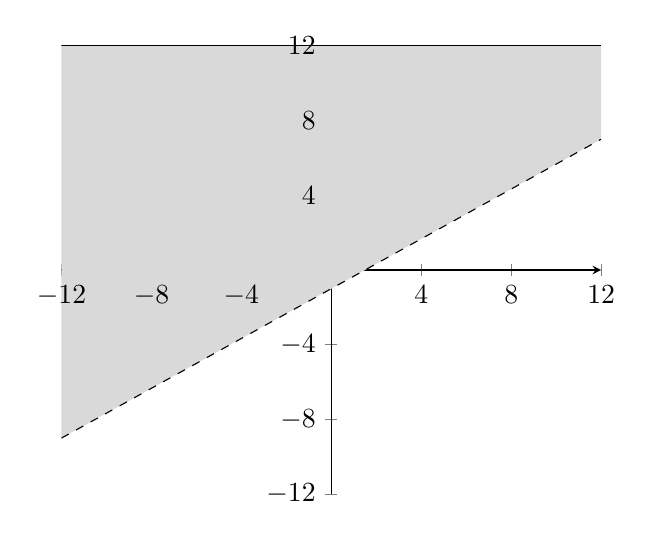
\begin{tikzpicture}
        \begin{axis}[xtick distance=4, ytick distance=4, xmin=-12, xmax=12, ymin=-12, ymax=12, axis x line=middle, axis y line=middle]
            \addplot[domain=-12:12,dashed, name path=plot]{2 / 3 *x - 1};
            \addplot[domain=-12:12,name path=top]coordinates {(-12,12) (12,12)};
            %\addplot[domain=-12:12,name path=bottom]coordinates {(-12,-12) (12,-12)};
            \addplot [gray!30] fill between [
            of=plot and top ];
        \end{axis}
    \end{tikzpicture}
    \begin{align*}
        \\
        \hspace{2cm}y &> \frac{2}{3}x - 1
        0 &> \frac{2}{3} \times 0 - 1\\
        0 &> 0 -1\\
        0 &> -1
    \end{align*}

    \subsection*{253}
    \hspace{3cm}
    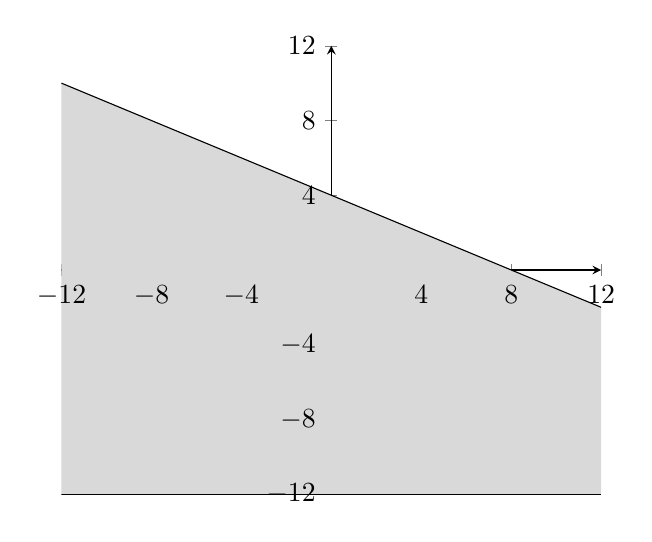
\begin{tikzpicture}
        \begin{axis}[xtick distance=4, ytick distance=4, xmin=-12, xmax=12, ymin=-12, ymax=12, axis x line=middle, axis y line=middle]
            \addplot[domain=-12:12, name path=plot]{-1 / 2 *x +4};
            %\addplot[domain=-12:12,name path=top]coordinates {(-12,12) (12,12)};
            \addplot[domain=-12:12,name path=bottom]coordinates {(-12,-12) (12,-12)};
            \addplot [gray!30] fill between [
            of=plot and bottom ];
        \end{axis}
    \end{tikzpicture}
    \begin{align*}
        \\
        \hspace{2cm}y \leq -\frac{1}{2}x + 4
    \end{align*}

    \subsection*{255}
    \hspace{3cm}
    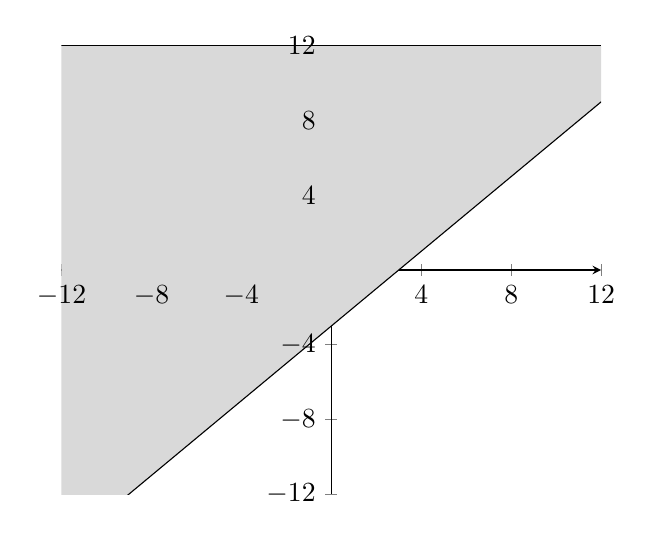
\begin{tikzpicture}
        \begin{axis}[xtick distance=4, ytick distance=4, xmin=-12, xmax=12, ymin=-12, ymax=12, axis x line=middle, axis y line=middle]
            \addplot[domain=-12:12, name path=plot]{x - 3};
            \addplot[domain=-12:12,name path=top]coordinates {(-12,12) (12,12)};
            %\addplot[domain=-12:12,name path=bottom]coordinates {(-12,-12) (12,-12)};
            \addplot [gray!30] fill between [
            of=plot and top ];
        \end{axis}
    \end{tikzpicture}
    \begin{align*}
        \\
        \hspace{2cm}x - y &\leq 3\\
        0 - 0 &\leq 3 \\
        0 &\leq 3
    \end{align*}

    \subsection*{257}
    \hspace{3cm}
    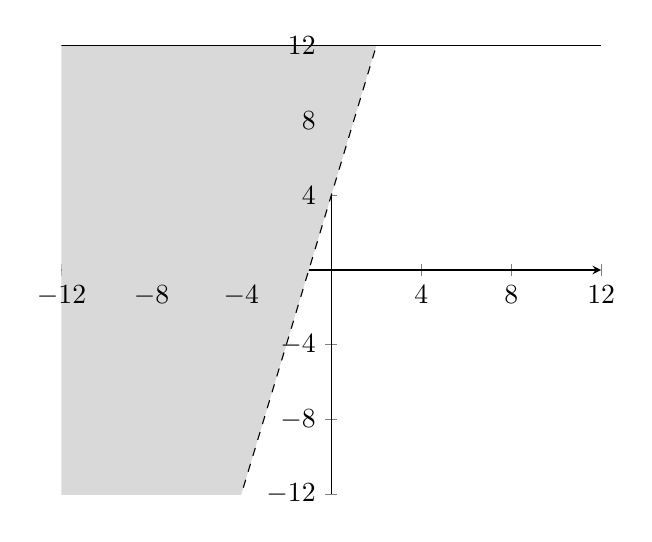
\begin{tikzpicture}
        \begin{axis}[xtick distance=4, ytick distance=4, xmin=-12, xmax=12, ymin=-12, ymax=12, axis x line=middle, axis y line=middle]
            \addplot[domain=-12:12, dashed, name path=plot]{4*x +4};
            \addplot[domain=-12:12,name path=top]coordinates {(-12,12) (12,12)};
            %\addplot[domain=-12:12,name path=bottom]coordinates {(-12,-12) (12,-12)};
            \addplot [gray!30] fill between [
            of=plot and top ];
        \end{axis}
    \end{tikzpicture}
    \begin{align*}
        \\
        \hspace{2cm}4x + y &> -4\\
        4 \times 0 + 0 &> -4\\
        0 + 0 &> -4\\
        0 &> -4)
    \end{align*}

    \subsection*{259}
    \hspace{3cm}
    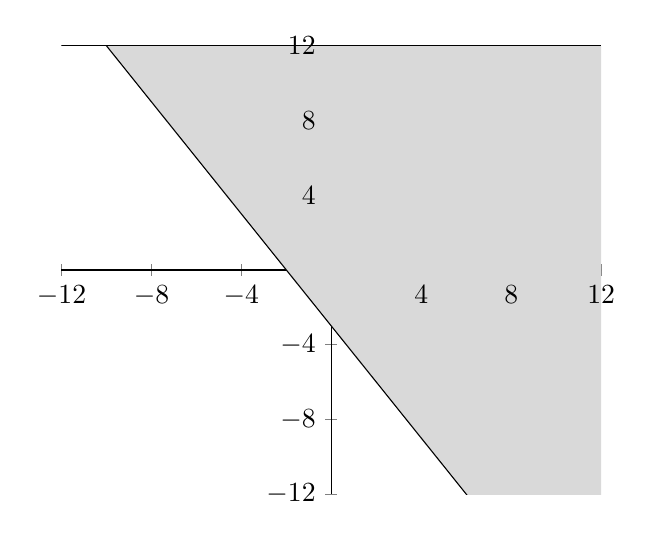
\begin{tikzpicture}
        \begin{axis}[xtick distance=4, ytick distance=4, xmin=-12, xmax=12, ymin=-12, ymax=12, axis x line=middle, axis y line=middle]
            \addplot[domain=-12:12, name path=plot]{-3 / 2 * x -3};
            \addplot[domain=-12:12,name path=top]coordinates {(-12,12) (12,12)};
            %\addplot[domain=-12:12,name path=bottom]coordinates {(-12,-12) (12,-12)};
            \addplot [gray!30] fill between [
            of=plot and top ];
        \end{axis}
    \end{tikzpicture}
    \begin{align*}
        \\
        \hspace{2cm}3x + 2y &\geq -6\\
        3 \times 0 + 2 \times 0 &\geq -6\\
        0 + 0 &\geq -6\\
        0 &\geq -6
    \end{align*}

    \subsection*{261}
    \hspace{3cm}
    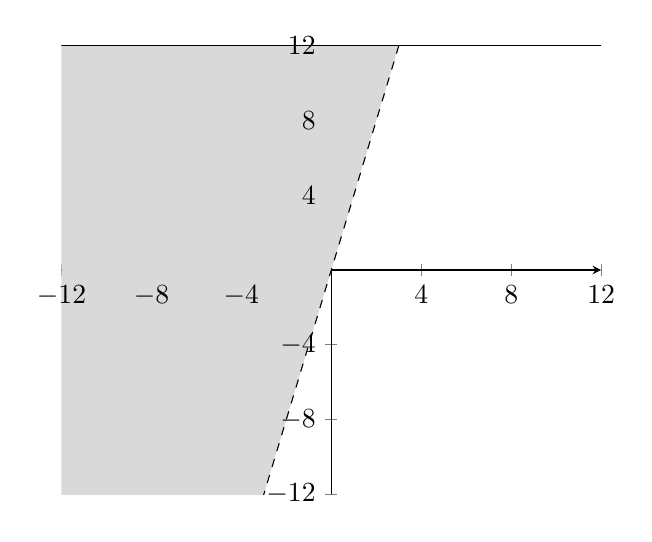
\begin{tikzpicture}
        \begin{axis}[xtick distance=4, ytick distance=4, xmin=-12, xmax=12, ymin=-12, ymax=12, axis x line=middle, axis y line=middle]
            \addplot[domain=-12:12, dashed, name path=plot]{x*4};
            \addplot[domain=-12:12,name path=top]coordinates {(-12,12) (12,12)};
            %\addplot[domain=-12:12,name path=bottom]coordinates {(-12,-12) (12,-12)};
            \addplot [gray!30] fill between [
            of=plot and top ];
        \end{axis}
    \end{tikzpicture}
    \begin{align*}
        \\
        \hspace{2cm} y &> 4x\\
        0 &> 4 \times -5 \\
        0 &> -5
    \end{align*}

    \subsection*{263}
    \hspace{3cm}
    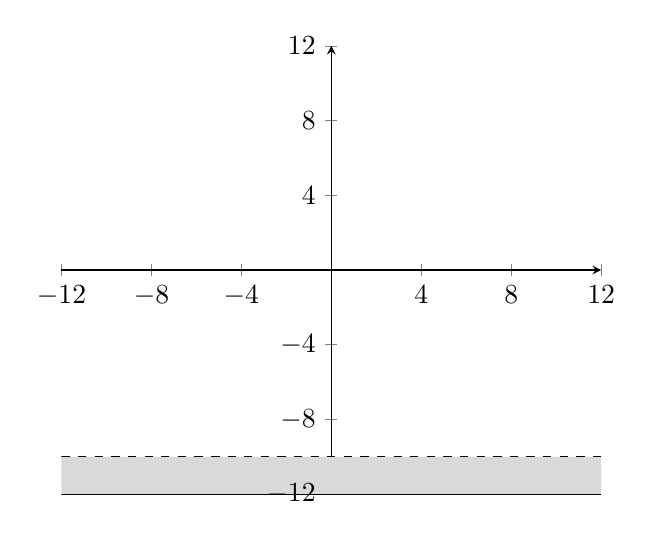
\begin{tikzpicture}
        \begin{axis}[xtick distance=4, ytick distance=4, xmin=-12, xmax=12, ymin=-12, ymax=12, axis x line=middle, axis y line=middle]
            \addplot[domain=-12:12, dashed, name path=plot]{-10};
            %\addplot[domain=-12:12,name path=top]coordinates {(-12,12) (12,12)};
            \addplot[domain=-12:12,name path=bottom]coordinates {(-12,-12) (12,-12)};
            \addplot [gray!30] fill between [
            of=plot and bottom ];
        \end{axis}
    \end{tikzpicture}
    \begin{align*}
        \\
        \hspace{2cm} y &< -10\\
    \end{align*}

    \subsection*{265}
    \hspace{3cm}
    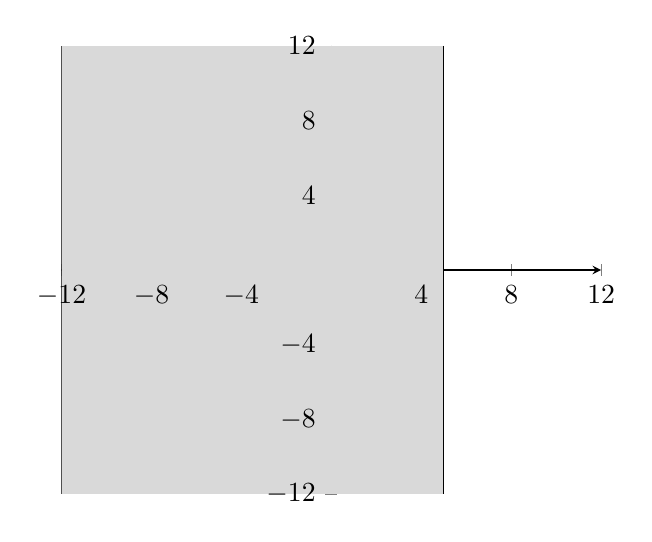
\begin{tikzpicture}
        \begin{axis}[xtick distance=4, ytick distance=4, xmin=-12, xmax=12, ymin=-12, ymax=12, axis x line=middle, axis y line=middle]
            \addplot[domain=-12:12, name path=plot]coordinates {(5,12) (5, -12)};
            \addplot[domain=-12:12,name path=left]coordinates {(-12,-12) (-12,12)};
            %\addplot[domain=-12:12,name path=top]coordinates {(-12,12) (12,12)};
            %\addplot[domain=-12:12,name path=bottom]coordinates {(-12,-12) (12,-12)};
            \addplot [gray!30] fill between [
            of=plot and left];
        \end{axis}
    \end{tikzpicture}
    \begin{align*}
        \\
        \hspace{2cm} x \leq 5 \\
    \end{align*}

    \subsection*{267}
    \hspace{3cm}
    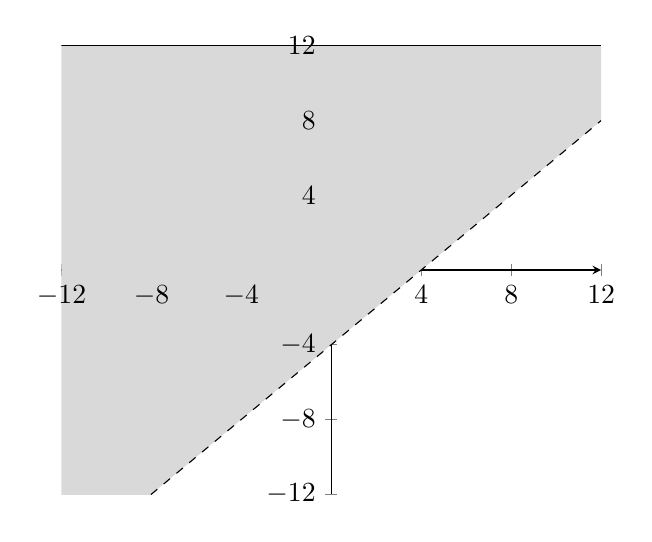
\begin{tikzpicture}
        \begin{axis}[xtick distance=4, ytick distance=4, xmin=-12, xmax=12, ymin=-12, ymax=12, axis x line=middle, axis y line=middle]
            \addplot[domain=-12:12, dashed, name path=plot]{x-4};
            %\addplot[domain=-12:12,name path=left]coordinates {(-12,-12) (-12,12)};
            \addplot[domain=-12:12,name path=top]coordinates {(-12,12) (12,12)};
            %\addplot[domain=-12:12,name path=bottom]coordinates {(-12,-12) (12,-12)};
            \addplot [gray!30] fill between [
            of=plot and top];
        \end{axis}
    \end{tikzpicture}
    \begin{align*}
        \\
        \hspace{2cm} x - y &< 4 \\
        0 - 0 &< 4 \\
        0 &< 4
    \end{align*}

    \subsection*{269}
    \hspace{3cm}
    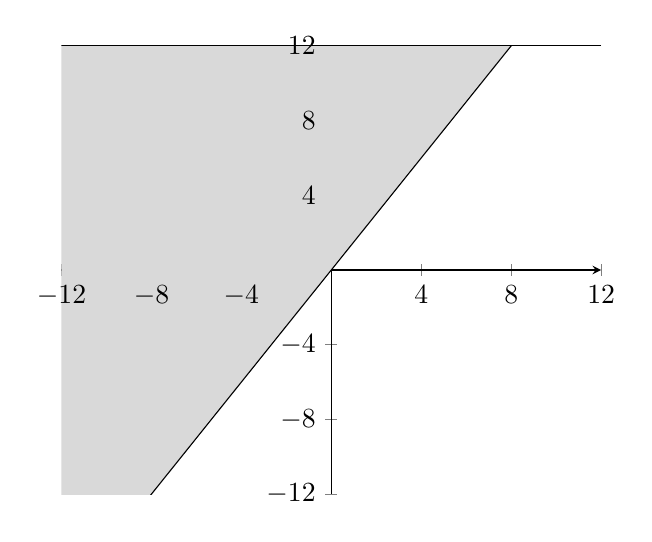
\begin{tikzpicture}
        \begin{axis}[xtick distance=4, ytick distance=4, xmin=-12, xmax=12, ymin=-12, ymax=12, axis x line=middle, axis y line=middle]
            \addplot[domain=-12:12, name path=plot]{3 / 2  *x};
            %\addplot[domain=-12:12,name path=left]coordinates {(-12,-12) (-12,12)};
            \addplot[domain=-12:12,name path=top]coordinates {(-12,12) (12,12)};
            %\addplot[domain=-12:12,name path=bottom]coordinates {(-12,-12) (12,-12)};
            \addplot [gray!30] fill between [
            of=plot and top];
        \end{axis}
    \end{tikzpicture}
    \begin{align*}
        \\
        \hspace{2cm} y &\geq \frac{3}{2}x \\
        4 &\geq 0\\
    \end{align*}

    \subsection*{271}
    \hspace{3cm}
    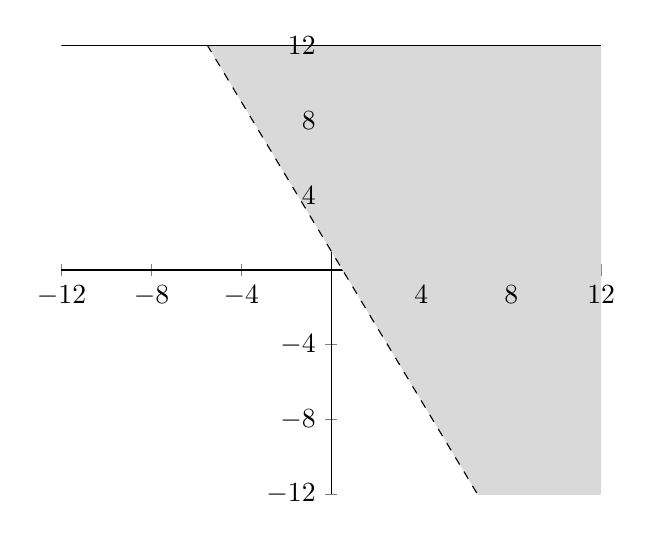
\begin{tikzpicture}
        \begin{axis}[xtick distance=4, ytick distance=4, xmin=-12, xmax=12, ymin=-12, ymax=12, axis x line=middle, axis y line=middle]
            \addplot[domain=-12:12, dashed, name path=plot]{-2*x +1};
            %\addplot[domain=-12:12,name path=left]coordinates {(-12,-12) (-12,12)};
            \addplot[domain=-12:12,name path=top]coordinates {(-12,12) (12,12)};
            %\addplot[domain=-12:12,name path=bottom]coordinates {(-12,-12) (12,-12)};
            \addplot [gray!30] fill between [
            of=plot and top];
        \end{axis}
    \end{tikzpicture}
    \begin{align*}
        \\
        \hspace{2cm} y &> -2x + 1 \\
        0 &> 0 + 1\\
        0 &> 1\\
    \end{align*}

    \subsection*{273}
    \hspace{3cm}
    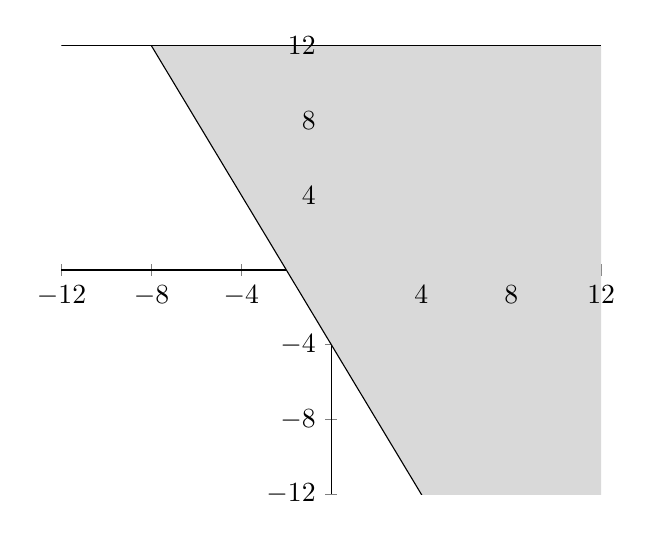
\begin{tikzpicture}
        \begin{axis}[xtick distance=4, ytick distance=4, xmin=-12, xmax=12, ymin=-12, ymax=12, axis x line=middle, axis y line=middle]
            \addplot[domain=-12:12, name path=plot]{-2*x - 4};
            %\addplot[domain=-12:12,name path=left]coordinates {(-12,-12) (-12,12)};
            \addplot[domain=-12:12,name path=top]coordinates {(-12,12) (12,12)};
            %\addplot[domain=-12:12,name path=bottom]coordinates {(-12,-12) (12,-12)};
            \addplot [gray!30] fill between [
            of=plot and top];
        \end{axis}
    \end{tikzpicture}
    \begin{align*}
        \\
        \hspace{2cm} 2x + y &\geq -4 \\
        0 &\geq -4\\
    \end{align*}

    \section*{3.5 283 to 327 odd}
    \subsection*{283 a}
        \begin{align*}
            Domain {(1,4), (2,8), (3,12), (4,16), (5,20) }\\
            \boxed{Domain = {1, 2, 3, 4, 5}}
        \end{align*}

    \subsection*{283 b}
    \begin{align*}
        Range {(1,4), (2,8), (3,12), (4,16), (5,20) }\\
        \boxed{Range = {4, 8, 12, 16, 20}}
    \end{align*}

    \subsection*{285 a}
    \begin{align*}
        Domain {(1,7), (5,3), (7,9), (-2,-3), (-2,8)}\\
        \boxed{Domain = {1, 5, 7, -2}}
    \end{align*}

    \subsection*{285 b}
    \begin{align*}
        Range {(1,7), (5,3), (7,9), (-2,-3), (-2,8)}\\
        \boxed{Range = {7, 3,  9, -3, 8}}
    \end{align*}

    \subsection*{287 a}
    \begin{align*}
        Ordered Pairs \\
        (Rebecca, January 18), \\
        (Jennifer, April 1),\\
        (John, January 18),\\
        (Hector, June 23),\\
        (Luis, February 15),\\
        (Ebony, April 7),\\
        (Raphael, November 6),\\
        (Meredith, August 19),\\
        (Karen, August 19),\\
        (Joseph, July 30)
    \end{align*}

    \subsection*{287 b}
    \begin{align*}
        Domain \\
        Rebecca \\
        Jennifer \\
        John \\
        Hector \\
        Luis \\
        Ebony \\
        Raphael \\
        Meredith \\
        Karen \\
        Joseph
    \end{align*}

    \subsection*{287 c}
    \begin{align*}
        Range \\
        January 18 \\
        April 1 \\
        June 23 \\
        February 15 \\
        April 7 \\
        November 6 \\
        August 19 \\
        July 30
    \end{align*}

    \subsection*{289 a}
    \begin{align*}
        Ordered Pairs \\
        (+100, 17.2)\\
        (110, 18.9)\\
        (120, 20.6)\\
        (130, 22.3)\\
        (140, 24.0)\\
        (150, 25.7)\\
        (160, 27.5)
    \end{align*}

    \subsection*{289 b}
    \begin{align*}
        Domain \\
        110 \\
        120 \\
        140 \\
        130 \\
        150 \\
        +100 \\
        160
    \end{align*}

    \subsection*{289 c}
    \begin{align*}
        Range \\
        18.9 \\
        27.5 \\
        20.6 \\
        22.3 \\
        24.0 \\
        25.7 \\
        17.2
    \end{align*}

    \subsection*{291 a}
    \begin{align*}
        &Ordered Pairs\\
        &(-3, 4), (-2, -1), (0, -3), (2, 3), (4, -1), (4, -3)
    \end{align*}

    \subsection*{291 b}
    \begin{align*}
        &Domain\\
        &{-3, -2, 0, 2, 4}
    \end{align*}

    \subsection*{293 c}
    \begin{align*}
        &Range\\
        &{-3, -1, 3, 4}
    \end{align*}

    \subsection*{293 a}
    \begin{align*}
        &Ordered Pairs\\
        &(-1, 4), (-1, -4), (0, 3), (0, -3), (1, 4), (1, -4)
    \end{align*}

    \subsection*{293 b}
    \begin{align*}
        &Domain\\
        &{-1, 0, 1}
    \end{align*}

    \subsection*{293 c}
    \begin{align*}
        &Range\\
        &{-4, -3, 3, 4}
    \end{align*}

    \subsection*{295 a}
    This is a function because there are no duplicate values in the domain
    \begin{align*}
        (-3, 9), (-2, 4), (-1, 1), (0, 0), (1, 1), (2, 4), (3, 9)
    \end{align*}

    \subsection*{295 b}
    \begin{align*}
        &Domain\\
        &-3, -2, -1, 0, 1, 2, 3
    \end{align*}

    \subsection*{295 c}
    \begin{align*}
        &Range\\
        &0, 1, 4, 9
    \end{align*}

    \subsection*{297 a}
    This is a function because there are no duplicate values in the domain
    \begin{align*}
        (-3, 27), (-2, 8), (-1, 1), (0, 0), (1, 1), (2, 8), (3, 27)
    \end{align*}

    \subsection*{297 b}
    \begin{align*}
        &Domain\\
        &-3, -2, -1, 0, 1, 2, 3
    \end{align*}

    \subsection*{297 c}
    \begin{align*}
        &Range\\
        &0, 1, 8, 27
    \end{align*}

    \subsection*{299 a}
        This is a function because there are no duplicate values in the domain\\


    \subsection*{299 b}
    \begin{align*}
        &Domain\\
        &-3, -2, -1, 0, 1, 2, 3
    \end{align*}

    \subsection*{299 c}
    \begin{align*}
        &Range\\
        &0, 1, 2, 3
    \end{align*}

    \subsection*{301 a}
        This is not function because there are duplicate values in the domain

    \subsection*{301 b}
    \begin{align*}
        &Domain\\
        &Jenny, Randy, Dennis, Emily, Raul
    \end{align*}

    \subsection*{301 c}
    \begin{align*}
        &Range\\
        &RHernandez@state.edu,\\
        &JKim@gmail.com, \\
        &Raul@gmail.com, \\
        &ESmith@state.edu,\\
        &DBrown@aol.com,\\
        &jenny@aol.com,\\
        &Randy@gmail.com
    \end{align*}

    \subsection*{303 a}
    \begin{align*}
        2x + y &= -3\\
        y &= -2x -3\\
        y &= -2 \times -1 - 3 \\
        y &= -1
    \end{align*}
    \hspace{4cm}This is a function

    \subsection*{303 b}
    \begin{align*}
        y &= x^2
    \end{align*}
    \hspace{4cm}This is a function

    \subsection*{303 c}
    \begin{align*}
        x + y^2 &= -5\\
        \cancel{x} + y^2 &= -x -5\\
        y^2 &= -x - 5
    \end{align*}
    \hspace{4cm}This is not a function

    \subsection*{305 a}
    \begin{align*}
        y - 3x^3 &= 2\\
        y \cancel{- 3x^3} &= 3x^3 + 2\\
        y &= 3x^3 + 2
    \end{align*}
    \hspace{4cm}This is a function

    \subsection*{305 b}
    \begin{align*}
        x + y^2 &= 3\\
        \cancel{x} y^2 &= -x + 3\\
        y^2 &= -x + 3
    \end{align*}
    \hspace{4cm}This is not a function

    \subsection*{305 c}
    \begin{align*}
        3x - 2y &= 6\\
        \cancel{3x} - 2y &= -3x +6\\
        - 2y &= -3x +6\\
        \frac{- 2y}{-2} &= \frac{-3x +6}{-2}\\
        y &= \frac{3}{2}x - 3
    \end{align*}
    \hspace{4cm}This is a function

    \subsection*{307 a}
    \begin{align*}
        f(x) &= 5x - 3\\
        f(2) &= 5 \times 2 - 3\\
        f(2) &= 7
    \end{align*}
    \begin{align*}
        \boxed{f(2) = 7}
    \end{align*}

    \subsection*{307 b}
    \begin{align*}
        f(x) &= 5x - 3\\
        f(-1) &= 5 \times -1 - 3\\
        f(-1) &= -8
    \end{align*}
    \begin{align*}
        \boxed{f(-1) = -8}
    \end{align*}

    \subsection*{307 c}
    \begin{align*}
        f(x) &= 5x - 3\\
        f(a) &= 5a- 3\\
    \end{align*}
    \begin{align*}
        \boxed{f(a) = 5a- 3}
    \end{align*}

    \subsection*{309 a}
    \begin{align*}
        f(x) &= -4x + 2\\
        f(2) &= -4 \times 2 + 2\\
        f(2) &= -6
    \end{align*}
    \begin{align*}
        \boxed{f(2) = -6}
    \end{align*}

    \subsection*{309 b}
    \begin{align*}
        f(x) &= -4x + 2\\
        f(-1) &= -4 \times -1 +2\\
        f(-1) &= 6
    \end{align*}
    \begin{align*}
        \boxed{f(-1) = 6}
    \end{align*}

    \subsection*{309 c}
    \begin{align*}
        f(x) &= -4x + 2\\
        f(a) &= -4a + 2\\
    \end{align*}
    \begin{align*}
        \boxed{f(a) = -4a + 2}
    \end{align*}

    \subsection*{311 a}
    \begin{align*}
        f(x) &= x^2 - x +3 \\
        f(2) &= 2^2 - 2 + 3\\
        f(2) &= 5
    \end{align*}
    \begin{align*}
        \boxed{f(2) = 5}
    \end{align*}

    \subsection*{311 b}
    \begin{align*}
        f(x) &= x^2 - x +3 \\
        f(-1) &= -1^2 + 1 +3\\
        f(-1) &= 5
    \end{align*}
    \begin{align*}
        \boxed{f(-1) = 5}
    \end{align*}

    \subsection*{311 c}
    \begin{align*}
        f(x) &= x^2 - x +3 \\
        f(a) &= a^2 - a + 3\\
    \end{align*}
    \begin{align*}
        \boxed{f(a) = a^2 - a + 3}
    \end{align*}

    \subsection*{313 a}
    \begin{align*}
        f(x) &= 2x^2 - x +3 \\
        f(2) &= 2 \times 2^2  - 2 + 3\\
        f(2) &= 9
    \end{align*}
    \begin{align*}
        \boxed{f(2) = 9}
    \end{align*}

    \subsection*{313 b}
    \begin{align*}
        f(x) &= 2x^2 - x +3 \\
        f(-1) &= 2 \times -1^2 + 1 +3\\
        f(-1) &= 6
    \end{align*}
    \begin{align*}
        \boxed{f(-1) = 6}
    \end{align*}

    \subsection*{313 c}
    \begin{align*}
        f(x) &= 2x^2 - x +3 \\
        f(a) &= 2a^2 - a + 3\\
    \end{align*}
    \begin{align*}
        \boxed{f(a) = 2a^2 - a + 3}
    \end{align*}

    \subsection*{315 a}
    \begin{align*}
        g(x) &= 2x +1 \\
        g(h2) &= 2h^2  +1\\
    \end{align*}
    \begin{align*}
        \boxed{g(h2) = 2h^2  +1}
    \end{align*}

    \subsection*{315 b}
    \begin{align*}
        g(x) &= 2x +1 \\
        g(x + 2) &= 2(x + 2) + 1\\
        g(x + 2) &= 2x + 4 + 1\\
        g(x + 2) &= 2x + 5\\
    \end{align*}
    \begin{align*}
        \boxed{ g(x + 2) = 2x + 5}
    \end{align*}

    \subsection*{315 c}
    \begin{align*}
        g(x) &= 2x +1 \\
        g(x) + g(2) &= 2x +1\\
        g(2) &= 2 \times 2 + 1\\
        g(2) &= 5\\
        g(x) + g(2) &= 2x +1 + 5\\
        g(x) + g(2) &= 2x +6
    \end{align*}
    \begin{align*}
        \boxed{f(a) = 2a^2 - a + 3}
    \end{align*}

    \subsection*{317 a}
    \begin{align*}
        g(x) &= -3x - 2 \\
        g(h2) &= -3h^2  -2
    \end{align*}
    \begin{align*}
        \boxed{g(h2) = -3h^2  -2}
    \end{align*}

    \subsection*{317 b}
    \begin{align*}
        g(x) &= -3x - 2 \\
        g(x + 2) &= -3(x + 2) - 2\\
        g(x + 2) &= -3x - 6 - 2\\
        g(x + 2) &= -3x - 8
    \end{align*}
    \begin{align*}
        \boxed{g(x + 2) = -3x - 8}
    \end{align*}

    \subsection*{317 c}
    \begin{align*}
        g(x) &= -3x - 2 \\
        g(x) + g(2) &= -3x - 2\\
        g(2) &= -3 \times 2 - 2\\
        g(2) &= -8\\
        g(x) + g(2) &= -3x - 2 -8\\
        g(x) + g(2) &= -3x - 10
    \end{align*}
    \begin{align*}
        \boxed{g(x) + g(2) = -3x - 10}
    \end{align*}

    \subsection*{319 a}
    \begin{align*}
        g(x) &= 3 - x \\
        g(h2) &= 3 - h^2
    \end{align*}
    \begin{align*}
        \boxed{g(h2) = 3 - h^2}
    \end{align*}

    \subsection*{319 b}
    \begin{align*}
        g(x) &= 3 - x \\
        g(x + 2) &= 3 - (x + 2)\\
        g(x + 2) &= 3 -x - 2\\
        g(x + 2) &= 1 - x
    \end{align*}
    \begin{align*}
        \boxed{g(x + 2) = 1 - x}
    \end{align*}

    \subsection*{319 c}
    \begin{align*}
        g(x) &= 3 - x \\
        g(x) + g(2) &=  3 - x\\
        g(2) &= 3 - 2\\
        g(2) &= 1\\
        g(x) + g(2) &= 3 - x + 1\\
        g(x) + g(2) &= 4 - x
    \end{align*}
    \begin{align*}
        \boxed{g(x) + g(2) = 4 - x}
    \end{align*}

    \subsection*{321}
    \begin{align*}
        f(x) &= 3x^2 - 5x\\
        f(2) &= 3 \times 2^2 - 5 \times 2\\
        f(2) &= 12 - 10\\
        f(2) &= 2\\
    \end{align*}
    \begin{align*}
        \boxed{f(2) = 2}
    \end{align*}

    \subsection*{323}
    \begin{align*}
        F(x) &= 2x^2 - 3x + 1\\
        F(-1) &= 2 \times -1^2 - 3 \times -1 + 1\\
        F(-1) &= 2 + 4\\
        F(-1) &= 6\\
    \end{align*}
    \begin{align*}
        \boxed{F(-1) = 6}
    \end{align*}

    \subsection*{325}
    \begin{align*}
        h(t) &= 2|t - 5| + 4\\
        h(-4) &= 2|-4 - 5| + 4\\
        h(-4) &= 2|-9| + 4\\
        h(-4) &= 18 + 4\\
        h(-4) &= 22
    \end{align*}
    \begin{align*}
        \boxed{h(-4) = 22}
    \end{align*}

    \subsection*{327}
    \begin{align*}
        f(x) & = \frac{x + 2}{x - 1}\\
        f(2) & = \frac{2 + 2}{2 - 1}\\
        f(2) & = \frac{4}{1}\\
        f(2) & = 4
    \end{align*}
    \begin{align*}
        \boxed{f(2) = 4}
    \end{align*}




\end{document}